\begin{figure}[H]
    \centering
    \begin{subfigure}{0.45\textwidth}
    \centering
    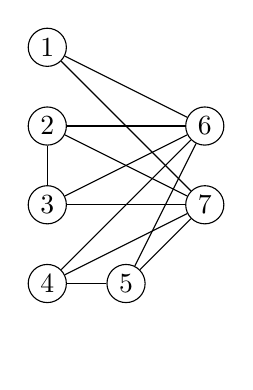
\begin{tikzpicture}[node distance=2cm, main node/.style={circle,draw,inner sep=2pt}]
        % Left Side
        \node[main node] (a) at ( 0, 4) [] {$1$};
        \node[main node] (b) at ( 0, 3) [] {$2$};
        \node[main node] (c) at ( 0, 2) [] {$3$};
        \node[main node] (d) at ( 0, 1) [] {$4$};
        
        % Right Side
        \node[main node] (e) at ( 2, 3) [] {$6$};
        \node[main node] (f) at ( 2, 2) [] {$7$};
        \node[main node] (g) at ( 1, 1) [] {$5$};
        
        % Edges
        \draw
            (a) edge (e)
            (a) edge (f)
            (b) edge (c)
            (b) edge (e)
            (b) edge (f)
            (c) edge (e)
            (c) edge (f)
            (d) edge (e)
            (d) edge (f)
            (d) edge (g)
            (g) edge (e)
            (g) edge (f);
            
            \useasboundingbox (0,0) rectangle (2,2.5);
    \end{tikzpicture}
    \caption{}
    \label{img:cograph:graph}
    \end{subfigure}
    \begin{subfigure}{0.45\textwidth}
    \centering
    \begin{tikzpicture}[node distance=2cm, 
        outer/.style={circle,draw,inner sep=1pt, minimum size=3.5mm}, 
        inner/.style={rectangle,draw}, 
        decoration={
            markings,
            mark=at position 0.5 with {\arrow{>}}}
    ]
        % Inner Nodes
        \node[inner] (a) at ( 0, 4) [] {$1$};
        \node[inner] (b) at ( 1, 3) [] {$0$};
        \node[inner] (c) at ( -1, 3) [] {$0$};
        \node[inner] (f) at ( -0, 2) [] {$1$};
        \node[inner] (g) at ( -1, 2) [] {$1$};
        
        % Outer Nodes
        \node[outer,font=\tiny] (h) at ( -2, 2) [] {$1$};
        
        \node[outer,font=\tiny] (i) at ( -1.25, 1) [] {$2$};
        \node[outer,font=\tiny] (j) at ( -0.75, 1) [] {$3$};
        \node[outer,font=\tiny] (k) at ( -0.25, 1) [] {$4$};
        \node[outer,font=\tiny] (o) at (  0.25, 1) [] {$5$};
        
        \node[outer,font=\tiny] (n) at ( 0.75, 2) [] {$6$};
        \node[outer,font=\tiny] (m) at ( 1.25, 2) [] {$7$};
        
        % Edges
        \draw
            % Inner Edges
            (a.south) edge (b.north)
            (a.south) edge (c.north)
            (b) edge (n)
            (b) edge (m)
            (c.south) edge (f.north)
            (c.south) edge (g.north)
            (c.south) edge (h.north)
            (g) edge (i)
            (g) edge (j)
            (f) edge (k)
            (f) edge (o);
            
            \useasboundingbox (0,0) rectangle (2,2.5);
    \end{tikzpicture}
    \caption{}
    \label{fig:cograph:cotree}
    \end{subfigure}
    
    \caption{    
    a) Example of a cograph with labeled nodes;
    b) Cotree trat represents the structure of the cograph \ref{img:cograph:graph}.
    \label{img:cograph}}
\end{figure}